\documentclass[border=3pt]{standalone}
\usepackage[T1]{fontenc}
\usepackage{helvet}
\renewcommand{\familydefault}{\sfdefault}
\usepackage{tikz}
\usetikzlibrary{arrows.meta,positioning,fit,backgrounds,shapes.geometric,calc}
\definecolor{ink}{HTML}{1F3A56}
\definecolor{core}{HTML}{DCE7F2}
\definecolor{know}{HTML}{DDEFE8}
\definecolor{game}{HTML}{F6E8D6}
\definecolor{model}{HTML}{EAE3F3}
\definecolor{plain}{HTML}{F3F4F6}
\definecolor{bad}{HTML}{B3402E}
\tikzset{
 every node/.style={font=\fontsize{8.5}{10.2}\selectfont,align=center,text=ink,execute at begin node={\hyphenpenalty=10000\exhyphenpenalty=10000}},
 box/.style={draw=ink,fill=white,rounded corners=1.5pt,minimum height=8.5mm,inner sep=3pt,line width=.5pt},
 corebox/.style={box,fill=core},
 knowbox/.style={box,fill=know},
 gamebox/.style={box,fill=game},
 modelbox/.style={box,fill=model},
 plainbox/.style={box,fill=plain},
 planned/.style={dashed},
 flow/.style={-{Stealth[length=2mm]},draw=ink,line width=.6pt},
 dflow/.style={flow,dashed},
 badflow/.style={flow,draw=bad,dashed},
 band/.style={draw=ink!55,rounded corners=3pt,inner sep=6pt,line width=.45pt},
 title/.style={font=\bfseries\fontsize{8.5}{10.2}\selectfont},
 lab/.style={font=\fontsize{7.5}{9}\selectfont,fill=white,inner sep=1pt},
 decision/.style={diamond,draw=ink,fill=core,aspect=2.1,inner sep=0.5pt,line width=.5pt}
}

\begin{document}
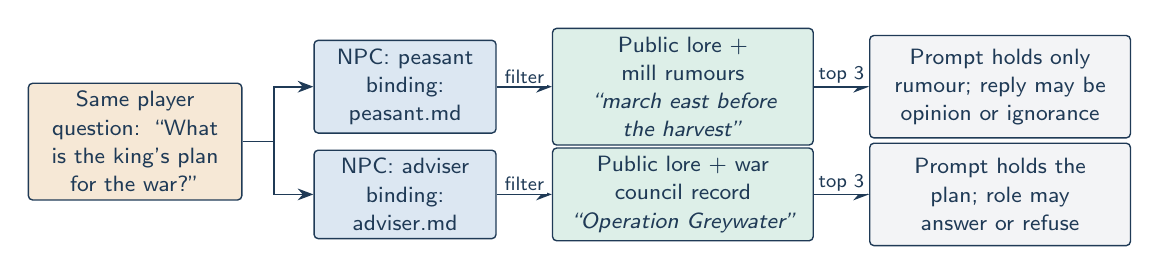
\begin{tikzpicture}
\node[gamebox,text width=25mm] (q) {Same player question: ``What is the king's plan for the war?''};
\node[corebox,text width=21mm,above right=1mm and 9mm of q.east,anchor=south west] (p) {NPC: peasant\\binding: peasant.md};
\node[corebox,text width=21mm,below right=1mm and 9mm of q.east,anchor=north west] (a) {NPC: adviser\\binding: adviser.md};
\node[knowbox,text width=31mm,right=7mm of p] (pd) {Public lore + mill rumours\\\emph{``march east before the harvest''}};
\node[knowbox,text width=31mm,right=7mm of a] (ad) {Public lore + war council record\\\emph{``Operation Greywater''}};
\node[plainbox,text width=31mm,right=7mm of pd,minimum height=13mm] (pr) {Prompt holds only rumour; reply may be opinion or ignorance};
\node[plainbox,text width=31mm,right=7mm of ad,minimum height=13mm] (ar) {Prompt holds the plan; role may answer or refuse};
\draw[flow] (q.east) -- ++(4mm,0) |- (p.west);
\draw[flow] (q.east) -- ++(4mm,0) |- (a.west);
\draw[flow] (p) -- node[lab,above] {filter} (pd);
\draw[flow] (a) -- node[lab,above] {filter} (ad);
\draw[flow] (pd) -- node[lab,above] {top 3} (pr);
\draw[flow] (ad) -- node[lab,above] {top 3} (ar);
\end{tikzpicture}
\end{document}
